\chapter{Analiza rozwiązań do automatycznej diagnostyki choroby Parkinsona}\label{ch:analiza-rozwiazan}


Diagnoza PD jest powszechnie oparta na obserwacjach lekarskich i ocenie objawów klinicznych, w tym charakterystyce różnorodnych objawów ruchowych.
Rosnąca liczba zachorowań i obniżenie wieku osób będących w grupie ryzyka, skutkuje wzrostem zainteresowania dotyczącym narzędzi, które ułatwiłyby
zarówno codzienne funkcjonowanie pacjentów jak i pracę lekarzy.
Tradycyjne metody diagnostyczne mogą być obarczone subiektywizmem ponieważ opierają się między innymi na ocenie ruchów, które są czasami subtelne dla
ludzkiego oka i dlatego trudne do sklasyfikowania, co może przyczynić się do błędnej diagnozy.
Ponadto wczesne objawy niemotoryczne PD mogą być łagodne oraz spowodowane wieloma innymi schorzeniami.
Dlatego też rozpoznanie tej choroby na wczesnym etapie stanowi wyzwanie.

Nie da się nie zauważyć, żę sztuczna inteligencja oraz nowoczesne technologie coraz częściej stają się integralną częścią systemu ochrony zdrowia.
Wspierają lekarzy podczas diagnozy oraz wyboru sposobu leczenia pacjenta, a także pozwalają na monitorowanie choroby.
Aby rozwiązać trudności i udoskonalić procedury diagnozowania oraz oceny PD, wdrożono metody uczenia maszynowego do klasyfikacji PD i osób zdrowych lub
pacjentów z podobnymi objawami klinicznymi (np. zaburzeniami ruchu lub innymi zespołami parkinsonowskimi).


Do roku 2020 powstało co najmniej 209 artykułów naukowych dotyczących wykorzystania metod uczenia maszynowego w diagnostyce i monitorowaniu \cite{ML_for_PD_review}
choroby Parkinsona, a liczba ta cały czas rośnie.


\section{Rodzaj wykorzystywanych danych}\label{sec:dane-przeglad}

Diagnozowanie choroby Parkinsona stanowi zadanie złożone ze względu na różnorodność objawów, które dotykają różne aspekty
funkcjonowania ciała i umysłu ludzkiego.
W związku z tym, techniki uczenia maszynowego wykorzystywane w tym obszarze, także skupiają się na różnych rodzajach danych.
Wśród tych źródeł informacji znajdują się wyniki badań obrazowych (np. rezonans magnetyczny - MRI, tomografia komputerowa - SPECT),
które wydają się intuicyjne, biorąc pod uwagę zmiany w aktywności mózgu, które można zaobserwować.
Niemniej jednak, istnieją także mniej oczywiste metody diagnozy, które budzą duże zainteresowanie w środowisku naukowym, szczególnie w początkowym stadium choroby.
Przykłady to analiza głosu, ocena charakterystyki chodu oraz badanie pisma odręcznego.

\begin{figure}[htbp]
	\centering
	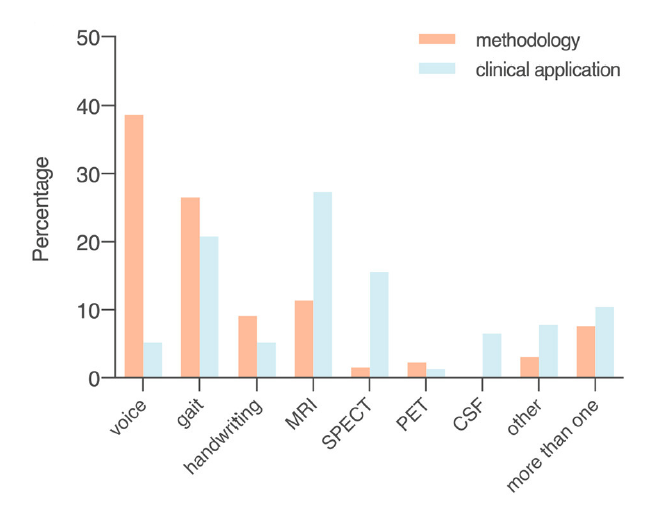
\includegraphics[width=0.5\textwidth]{./img/plot_PD_detection_methods}
	\caption{Wykres przedstawiający rozkład rodzaju danych na których bazowały systemy ML do diagnostyki PD (stan na dzień 14 luty 2020) \cite{ML_for_PD_review} }
    \label{fig:pd_detection_methods}\label{fig:figure}
\end{figure}

Rysunek \ref{fig:pd_detection_methods} ilustruje zastosowanie wymienionych metod zarówno w teorii, jak i praktyce.
Metody oparte na obrazowaniu medycznym wykazują wyraźną przewagę w zastosowaniach klinicznych w porównaniu do kontekstu teoretycznego.
Niemniej jednak, to pozostałe metody budzą znacznie większe zainteresowanie ze strony środowiska naukowego.
Szczególnie w przypadku analizy głosu, gdzie rozbieżność między teorią a praktyką jest szczególnie znacząca.
Przyczyny tego zjawiska zostaną dokładniej rozważone w kolejnych fragmentach.

Niniejsza praca dotyczy diagnostyki na podstawie głosu, dlatego ten temat zostanie rozwinięty.
Założeniem dla takich systemów jest zadanie potencjalnemu pacjentowi zadania wokalnego, może to być:
\begin{itemize}[itemsep=0.1pt]
	\item podtrzymywane samogłoski (ang. \emph{sustained vowels}),
	\item zadanie diadochokinetyczne (DDK), mogące mierzyć zdolność do wydawania serii szybkich i naprzemiennych dźwięków (sylab),
	\item czytanie tekstu,
	\item wypowiedzenie pojedynczego zdania,
	\item monolog.
\end{itemize}

Dotychczas nie przeprowadzono badań porównawczych dotyczących wpływu wyboru zadania wokalnego na efektywność klasyfikacji w przypadku choroby Parkinsona (PD).
Jedynie w artykule  \cite{vocal_task_comparision} przeprowadzono takie porównanie, przy użyciu cech prozodii.
Nie pozwala to jednak na wyciągnięcie obiektywnych wniosków, ponieważ każde z zadań wokalnych może wymagać innego podejścia i metod klasyfikacji.
Niemniej jednak, autorzy publikacji \cite{monitoring_speech} przeprowadzili badanie na 200 pacjentach z PD,
gdzie dokonano klasyfikacji deficytów mowy na pięć poziomów nasilenia.
Oceniono typ (głos, artykulacja, płynność) oraz zakres upośledzenia dla każdego poziomu, korzystając z 2-minutowego fragmentu mowy.
Wyniki ukazały, że głos stanowił najczęściej występujący i bardziej nasilony deficyt we wczesnych stadiach choroby.
Deficyty artykulacji i płynności pojawiały się później.
Wykazano, że upośledzenie artykulacji korelowało z upośledzeniem głosu w fazie "ciężkiej", a w fazie "głębokiej" dominującą cechą była upośledzona artykulacja.

W rezultacie, w kontekście wczesnej diagnostyki choroby, artykulacja i płynność mowy nie wymagają głębokiej uwagi.
Koncentrację należy skupić przede wszystkim na cechach głosowych, co sprawia, że wybór podtrzymywanych samogłosek jako zadania wokalnego
wydaje się być najlepszym wyborem ze względu na ich stabilność w czasie oraz łatwość wypowiadania przez pacjenta.
To podejście może posiadać potencjał uniwersalności dla różnych języków, co oznacza, że analiza może być stosowana
niezależnie od języka ojczystego pacjenta.
W efekcie pozwala to na bardziej efektywne i znormalizowane diagnozowanie choroby Parkinsona.

%---------------------------------------------------------------------------

\section{Metody klasyfikacji}\label{sec:metody-klasyfikacji}

W zależności od przyjętego podłoża diagnostycznego dobiera się odpowiednią metodę klasyfikacji.
Różne metody okażą się skuteczne w przypadku analizy mowy spontanicznej w porównaniu do mowy kontrolowanej.
W tej sekcji zostaną przedstawione metody klasyfikacji związane z podtrzymywaniem samogłosek, które to zostały wybrane jako
fundament badawczy w ramach niniejszego opracowania.



In this research paper, we set forward a new approach based on speech signal analysis for PD detection. The main novelty of our approach resides
in the extraction of new features which have not yet been extracted from the used dataset, called i-vector features and CNN
deep features. We extracted from each voice sample three i-vectors
of different sizes 100, 200, and 300 using Gaussian Mixture Models (GMM) based on Universal Background Model (UBM) applied
on 39-dimensional Mel-Frequency Cepstral Coefficients (MFCC). As
a matter of fact, three different models were obtained after using
i-vector features and raw signal values as inputs for both learning
techniques, namely CNN and SVM. Finally, we calculated the accuracy, precision, recall/sensitivity, specificity and f -score for each
model in order to assess its performance in terms of PD detection. \cite{2023_PD_voice}

%---------------------------------------------------------------------------

\section{Wyzwania związane z systemami automatycznej diagnostyki}\label{sec:wyzwania}

Zainteresowanie systemami do automatycznej diagnostyki choroby Parkinsona na podstawie głosu jest ogromne i wiąże się z nim duże nadzieje.
Istnieje jednak duża dysproporcja pomiędzy pracą badawczą a ich wykorzystaniem w rzeczywistym środowisku Rys \ref{fig:pd_detection_methods}.
Przyczyn takiego stanu rzeczy jest wiele, a większość z nich związana jest z brakiem usystematyzowanego podejścia do problemu, co utrudnia porównanie
rozwiązań, a tym samym rzetelny postęp.

Ostatnie badania wykazały, że możemy wytrenować dokładne modele do wykrywania oznak PD z nagrań audio.
Jednakże, istnieją rozbieżności, które są częściowo powodowane przez różnice w
wykorzystywanych korpusach lub metodologii.
Dlatego autorzy publikacji \cite{SustainedVowelsProblems} przeprowadzili analizę, wpływu niektórych czynników na wyniki klasyfikacji.
Głównym celem artykułu była ich identyfikacja oraz stworzenie zasad, które w przyszłości pozwolą usystematyzować
stan wiedzy w tej dziedzinie.
W badaniach skupiono się na przedłużonych samogłoskach (ang. \emph{sustained vowels}), ponieważ są one najlepszym i najpopularniejszym zadaniem
wokalnym w takich systemach.
Przeprowadzone eksperymenty wykazały, że nieuwzględnione zmienne w metodologii, projekcie eksperymentalnym i
przygotowaniu danych prowadzą do zbyt optymistycznych wyników w badaniach nad automatyczną detekcją PD.
Czynniki, które zidentyfikowano jako przyczyniające się do zbyt optymistycznych wyników klasyfikacji
przedstawiono na Rys. \ref{fig:factors_PD_detection} oraz omówiono poniżej.


\begin{figure}[htbp]
	\centering
	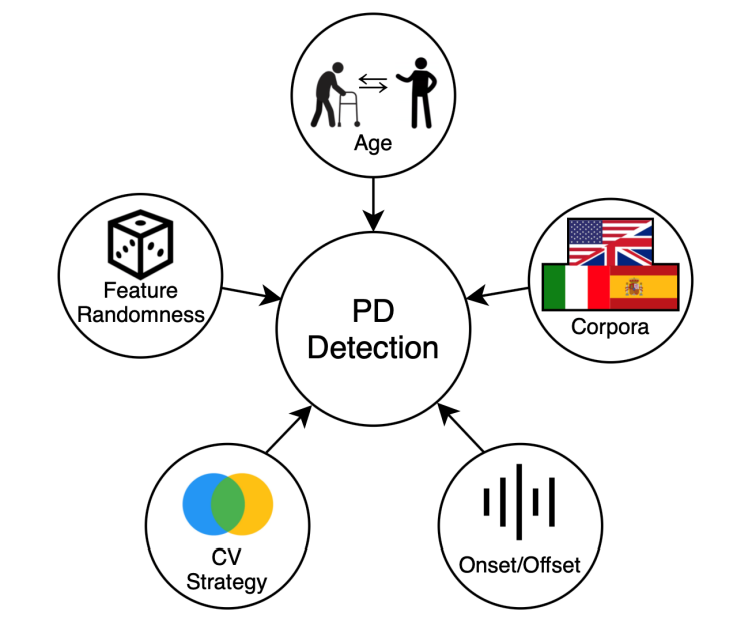
\includegraphics[width=0.4\textwidth]{./img/influence_of_factors_on_PD_detection}
	\caption{Czynniki wpływające na dokładność detekcji PD na podstawie głosu \cite{SustainedVowelsProblems}}
    \label{fig:factors_PD_detection}
\end{figure}


\begin{enumerate}[label={\alph*)}]
	\item \textbf{Pominięcie aspektu tożsamości mówcy przy konstruowaniu zbiorów treningowych i testowych}
	\item[] W przypadku, gdy w zbiorze danych znajduje się kilka nagrań od tego samego mówcy można postąpić na dwa sposoby.
Pierwszy z nich to podział według podmiotów (ang. \emph{subject-wise split}) polegający na tym, że nagrania od tej samej
osoby znajdują się albo w zbiorze treningowym albo testowym - nigdy w obu na raz.
Drugie podejście to podział według rekordów (ang. \emph{record-wise split}), gdzie nagrania są losowo dzielone do zbiorów
lub intencjonalnie używa się nagrań od tej samej osoby zarówno w zbiorze testowym jak i treningowym.
Okazuje się, że podejście typu \emph{record-wise} prowadzi do wyższej dokładności niż \emph{subject-wise split}, jeśli pozostałe założenia pozostają identyczne.
Prawdopodobnie wynika to z faktu, że klasyfikator nastawia się na wykrywanie unikalnych informacji indywidualnych,
reprezentowanych przez współczynniki takie jak MFCC, a nie rzeczywiste biomarkery lub wzorce PD.
Dlatego też rekomendowana jest technika \emph{subject-wise split}, aby uniknąć zbyt optymistycznych wyników.

  	\item \textbf{Niezbalansowanie klas pod względem wieku}
	\item[] W literaturze można znaleźć prace wykorzystujące zbiory danych, w których średni wiek mówców
w klasie osób chorych na PD różni się od średniego wieku w klasie osób zdrowych o ponad 5 lat.
Autorzy zapewniają o wysokiej skuteczności swoich rozwiązań, jednak pomijają informacje o ryzyku, że klasyfikator
uczy się wykrywać cechy powiązane z wiekiem, zamiast rzeczywistych wzorców PD.
Wyniki eksperymentów w publikacji \cite{SustainedVowelsProblems} pokazują, że wraz ze wzrostem różnicy między średnim wiekiem uczestników z PD i HC,
dokładność klasyfikacji konsekwentnie rośnie (Rys. \ref{fig:acc_and_age_diff}).
Na tej podstawie można stwierdzić, że związany z wiekiem wpływ na głos mówców może zaburzać wyniki otrzymywane przez klasyfikator.
Dlatego też zaleca się zbalansowanie używanych zbiorów danych, tak aby średnia różnica wieku między tymi dwoma klasami była jak namniejsza.


\begin{figure}[htbp]
	\centering
	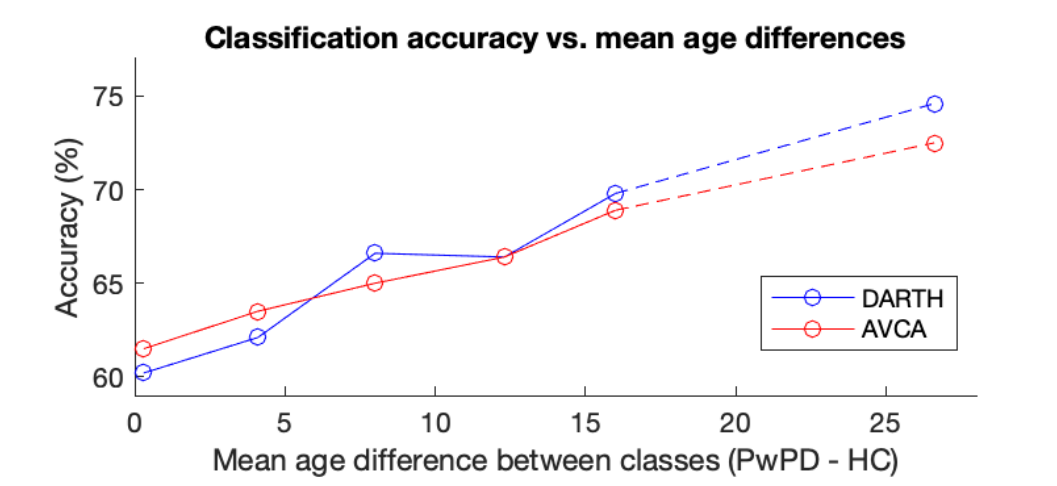
\includegraphics[width=0.7\textwidth]{./img/acc_and_age_difference}
	\caption{Wykres przedstawiający zależność różnicy wieku między klasami a dokładnością klasyfikacji \cite{SustainedVowelsProblems}}
    \label{fig:acc_and_age_diff}
\end{figure}

  	\item \textbf{Wpływ losowości cech na dokładność klasyfikacji}
	\item[] W publikacji \cite{SustainedVowelsProblems} przeprowadzono badania analizujące wpływ losowości cech na dokładność klasyfikacji.
Zamieniono cechy obliczone za pomocą DARTH-VAT na losowe liczby, zachowując etykiety i podziały.
Wyniki wskazały, że nawet losowe cechy mogą prowadzić do wysokich wyników klasyfikacji (ponad 72\%).
Efekt ten jest bardziej widoczny w mniejszych korpusach, gdzie różnica między liczbą nagrań a wymiarowością cech ma większy wpływ na potencjalną korelację przypadkową.
Badanie pokazuje, że nadmierna liczba cech w stosunku do liczby obserwacji może prowadzić do fałszywie wysokich wyników klasyfikacji nawet przy użyciu losowych cech.
Im większa różnica między liczbą plików a wymiarem wektora cech, tym większe szanse na znalezienie cechy, która losowo koreluje z etykietami klas.
To sugeruje, że osiągnięcia klasyfikacyjne powinny być analizowane w kontekście proporcji cech do próbki, aby uniknąć nadmiernie optymistycznych interpretacji wyników klasyfikacji w zastosowaniach medycznych.

  	\item \textbf{Ograniczenie losowego nadmiernego dopasowania poprzez uwzględnienie zbioru walidacyjnego}
	\item[] Dla mniejszych zbiorów danych, praktyką jest często używanie tylko zbiorów treningowych i testowych podczas krzyżowej walidacji.
Jest to podejście, które może prowadzić do wyników zbyt optymistycznych, ponieważ wszystkie wyniki testowe są brane pod uwagę przy wyborze optymalnej
konfiguracji modelu.
Inną strategią jest wykorzystanie danych treningowych do oceny wytrenowanych modeli i późniejsze przetestowanie najlepszego modelu na zbiorze testowym.
Niemniej jednak, to podejście może być niepraktyczne, ponieważ może prowadzić do wyników idealnych (dokładność 100\%) na zbiorze treningowym, co jest niepożądane.
Aby uniknąć tych problemów, proponuje się wykorzystanie dodatkowego zbioru walidacyjnego \cite{SustainedVowelsProblems}.
Wybierając model na podstawie wyników walidacyjnych, a następnie testując go na zbiorze testowym, można uniknąć ryzyka nadmiernego dopasowania.
Dla mniejszych zbiorów danych, ta strategia może ograniczać dostępną liczbę danych treningowych, co wpływa na wydajność klasyfikacji.

	\item \textbf{Wpływ początku i końca  nagrań samogłosek na wyniki klasyfikacji}
\item[] Główną różnicą między korpusami wykorzystywanymi do klasyfikacji choroby Parkinsona (PD) jest obecność fragmentów nagrania oznaczonych jako "onset" i "offset".
Niektóre nagrania zawierają te segmenty, podczas gdy inne zostały ich pozbawione, aby zapewnić stabilniejszą fonację, co jest korzystne dla pewnych cech i algorytmów analizy.
W celu oceny znaczenia informacji zawartych w obszarach "onset" i "offset" dla klasyfikacji, przeprowadzono eksperymenty porównawcze,
wykorzystując nagrania zarówno z fragmentami przyciętymi, jak i nieprzyciętymi \cite{SustainedVowelsProblems}.
Wyniki tych eksperymentów ukazały, że wyeliminowanie fragmentów początkowych i końcowych wpłynęło negatywnie na dokładność klasyfikacji.
To wskazuje na to, że obszary te zawierają istotne informacje artykulacyjne, które mają znaczenie dla procesu klasyfikacji.

 	\item \textbf{Eksperymenty międzykorporowe a zdolności generalizacyjne}
	\item [] Większość badań dotyczących diagnozowania choroby Parkinsona na podstawie głosu opiera się na jednym, lub ewentualnie kilku (wykorzystywanych niezależnie)
korpusach mowy.
W tym kontekście często pomija się badanie zdolności klasyfikatorów do ogólnego zastosowania.
W artykule \cite{SustainedVowelsProblems} przeprowadzono międzykorporowe eksperymenty na bazach danych w językach włoskim i hiszpańskim w celu
przetestowania zdolności ogólnych modeli. Skuteczność tych modeli różniła się w zależności od języka zbioru testowego.
Może to wynikać z odmiennej różnorodności nagrań, co ma wpływ na stabilność modelu.
Drugim możliwym wyjaśnieniem jest to, że głos osób z chorobą Parkinsona może być w różnym stopniu obarczony objawami choroby w zależności od języka ojczystego lub stopnia zaawansowania choroby.
Innymi słowy, w zależności od użytego zbioru danych objawy mogą być nasilone w różny sposób i konieczne jest wzięcie tego pod uwagę tak by zdolności generalizacyjne modelu były jak najwyższe.
\end{enumerate}


Identyfikacja i świadomość wpływu powyższych czynników, pozwala na dostosowaniu przeprowadzanych ekperymentów tak, aby uniknąć wyników zbyt optymistycznych.
Usystematyzowanie podejścia do analizy głosu pod kątem diagnostyki choroby Parkinsona przyczyni się do możwliwości obiektywnego porównania istniejących i nowych rozwiązań.
Tym samym przyspiesy to postęp w tej dziedzinie i uzyskanie optymalnego rozwiązania, które mogłoby zostac wykorzystane w rzeczywistym środowisku.

Nie są to jednak wszystkie czynniki, które zaburzają obiektywność wyników. Konieczna jest dyskusja na temat nowych
kompleksowych linii bazowych dla prowadzenia eksperymentów w automatycznym wykrywaniu PD na podstawie fonacji,
a także innych ogólnych zastosowań przetwarzania mowy.

Prace nad automatyczną detekcją Parkinsona na podstawie głosu trwają już od dłuższego czasu.
Jednak wciąż brakuje systemu, który mógłby zostać uznany jako wystarczajaco niezawodne narzędzie diagnostyczne.
Wśród problemów, które ograniczają rzeczywiste wykorzystanie takich systemów wyróżnia się:

[https://parkinsonsnewstoday.com/news/speech-analysis-can-help-detect-parkinsons-in-early-stages-study-says/]

Techniques that analyze speech and vocal patterns might be effective tools to diagnose Parkinson’s disease, and possibly at earlier stages than is now possible, according to a new study.

There are no laboratory biomarkers that can detect Parkinson’s, and brain imaging scans do not allow for a definitive diagnosis. The clinical diagnosis of the disease is currently based on the manifestation of two to three motor symptoms, including muscle stiffness, resting tremor, slowness of movement and balance issues.

These criteria can identify Parkinson’s with 90% accuracy, but it takes, on average, 2.9 years to reach a diagnosis.

Speech is a complicated skill, and it’s often affected by Parkinson’s-associated motor changes. Between 60 and 80% of patients may experience reduced vocal loudness, harsh or breathy vocal quality and abnormal speaking rates. For that reason, a team of researchers at three centers — Universidad Politécnica de Madrid, Massachusetts Institute of Technology and Johns Hopkins University — is working to develop a digital diagnostic tool for Parkinson’s disease based on the voice.

In the study “Analysis of speaker recognition methodologies and the influence of kinetic changes to automatically detect Parkinson’s Disease,” published in Applied Soft Computing, researchers tested various speaker recognition techniques for their ability to identify Parkinson’s disease in a database of Spanish-language speech.

Results build on past work by the team, and continues to demonstrate that speech carries information relevant to an accurate and differential diagnosis of Parkinson’s. It also shows that speech features of interest can be automated and assessed, with diagnostic reliability.

The team had previously found that a speech analysis technique, called RASTA-PLP, had an 82% accuracy in automatically identifying Parkinson’s patients. This study uses a further refinement of the RASTA-PLP technique, and identified patients voices with 87% accuracy.

“The early detection of Parkinson along with the anticipation of the start of treatment would have a relevant effect on both the quality of life of patients and the healthcare system. This would allow us to develop new therapies and better understand the disease and its evolution,” Juan Ignacio Godino, a researcher from Universidad Politécnica and a study co-author, said in a news release.

This research is ongoing, and scientists are currently enrolling patients in studies. If you are 45-90 years of age, do not suffer from and do not have a family history of Parkinson’s, you could consider joining the study. A contact form (in Spanish) can be found here.


Inne

* https://voicefoundation.org/health-science/voice-disorders/voice-disorders/voice-dysfunction-in-neurological-disorders/parkinsons-disease/

%---------------------------------------------------------------------------
